\documentclass{report}

\usepackage{biblatex}
\addbibresource{../../Resources/resources.bib}

\usepackage{graphicx}
\usepackage{tikz}
\usetikzlibrary{arrows}
\usetikzlibrary{quantikz}

\usepackage{physics}
\usepackage{amsthm}
\usepackage{amsfonts}

\newtheorem{definition}{Definition}
\newtheorem{theorem}{Theorem}
\newtheorem{problem}{Problem}
\newtheorem{lemma}{Lemma}

\title{Bridging gates over qubits}
\author{Seyed Sajad Kahani \\ 22222815 \\Supervisor: Prof. Dan Browne}
\date{\today}
\begin{document}
\maketitle

\tableofcontents

\begin{abstract}
  
\end{abstract}

\chapter{Introduction}

Quantum computation is an emerging field that aims to use quantum mechanics to solve problems that are intractable for classical computers. Since the earliest conceptualization of quantum computation~\cite{feynman1986}, it has been believed that quantum computers could revolutionize the way we solve problems, particularly those involving simulating nature. Over time, it has become clear that quantum computers have applications far beyond physical simulations. There are algorithms for search and traversing graphs, solving linear equations~\cite{montanaro2016}, and methods for machine learning and optimization~\cite{jordan2023}.

Despite significant efforts, we are still far from fully utilizing these algorithms. Our current hardware technology has not yet achieved the desired accuracy and number of qubits necessary for quantum computers to outperform classical computers in solving useful problems. The current situation is commonly referred to as the ``noisy intermediate scale quantum'' (NISQ) era~\cite{preskill2018}, characterized by restricted resources, including a limited number of qubits, constrained qubit connectivity, hardware-specific gate sets, and limited circuit depth due to noise \cite{TODO}.
% https://www.epfl.ch/labs/lsi/fereshte-research/ 

The restricted qubit resources and excessive noise susceptibility of NISQ devices necessitate optimal compilers to have any hope of useful near-term quantum computation. A huge amount of research has been conducted to tackle different aspects of the compilation problem, including qubit allocation \cite{TODO}, routing \cite{TODO}, scheduling \cite{TODO}, and gate synthesis \cite{TODO}. These aspects are deeply intertwined and one may not distinguish between them, but all of them are in some sense a circuit transformation from a higher-level circuit (with fewer imposed constraints) to a lower-level circuit (with more imposed constraints) \cite{TODO}.

While the knowledge of classical compilation is adopted and the divergent points (no-cloning \cite{TODO} and reversibility \cite{TODO}) are studied and addressed well, another important distinction has received less attention - the cost of SWAP operations. In classical circuit synthesis, SWAPs simply rearrange wires at negligible cost, compared to two-bit gates. But in the quantum realm, SWAP gates require double entangling \cite{TODO} interactions between qubits, making them the most expensive two-qubit quantum logic gates \cite{TODO}.

Despite extensive research into minimizing the overall number of SWAP operations~\cite{childs, TODO}, there is little work addressing the inherent cost of each SWAP gate. A few recent works have proposed techniques to reduce the cost of SWAP gates, such as embedding SWAPs within other 2-qubit gates in 2QAN compiler~\cite{lao2021}, or optimization of SWAP decompositions into CNOT gates~\cite{kissinger2019,nash2020}. In this work, we aim to address the primary usage of SWAP gates - enabling connectivity between non-adjacent qubits. We analyze the possibility of simplifications for different connectivity cases.

Here we define a problem called bridging that is to find a circuit that applies a two-qubit gate on two non-adjacent qubits. By utilizing the framework of~\cite{kissinger2019} and the extensive literature of network coding \cite{TODO} show that in the classical case, the cost of bridging over $n$ bits is $4n$ to $6n$ (upto a $O(1)$ constant). We also present a circuit that achieves the lower bounds. We then attempt to extend the results to the quantum regime, by presenting a circuit to bridge two-qubit gates with Schmidt number $2$ over $n$ with optimal number of CNOTs.

This advancement will lead to $33\%$ reduction in the cost of the most expensive two-qubit gate in many situations. To demonstrate the practicality of our results, we implement the algorithms and benchmark with application-oriented dataset of circuits.

The rest of this thesis is organized as follows. Chapter~\ref{chap:related_works} reviews the related works. In Chapter~\ref{chap:discussion}, we present the algorithms and prove their correctness and optimality for the classical and quantum cases. We implement the algorithms and benchmark against state-of-the-art techniques in Chapter~\ref{chap:implementation}. Finally, Chapter~\ref{chap:conclusion} concludes and discusses avenues for future work.

\chapter{Related Works}\label{chap:related_works}

TODO:
\begin{itemize}
  \item Hamiltonian compilers (not anymore) \cite{lao2021,campbell2019,childs2021}
  \item Classical Compilers (not anymore)
  \item General-purpose quantum compilers \cite{cross2022,sivarajah2021,qiskit2023,maronese2021}
  \item Papers with a focus on inital mapping \cite{siraichi2018,zhang2021,paler2019}
  \item Papers with a focus on routing problem \cite{childs,zhou2020,itoko2019,cowtan2019}
  \item Ideas to improve SWAP complexity (embedding from 2QAN and CNOT framework from Kissinger) \cite{lao2021}\cite{nash2020,kissinger2019}
  \item Papers with a focus on decomposition of gates and KAK (maybe) \cite{tucci2005,vatan2004a}
  \item Papers with a focus on entangling power (maybe) \cite{nielsen2003,berry2002,bennett2002,linowski2020}
  \item A bit from Network coding \cite{ho2008}
\end{itemize}


\chapter{Discussion}\label{chap:discussion}

It is a well-known fact that a SWAP gate could not be decomposed to less than three CNOTs. For a more complex circuit involving a SWAP or more, this does not necessarily hold in general, especially in presence of connectivity contraints. Here we provide two examples (\ref{ex:swap-swap-decomposition} and \ref{ex:cnot-bridge-decomposition}) with linear connectivity constraints of SWAPs that are used to apply a two-qubit gate on non-adjacent qubits.
They show that decomposing SWAPs to three CNOTs will not necessarily lead to an optimal circuit, even in simple cases.

\begin{figure}[ht]
  \centering
  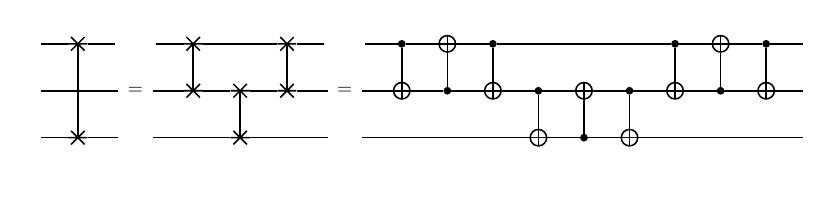
\begin{tikzpicture}
  \node[scale=0.7] {
  \begin{quantikz}
    \qw & \swap{2} & \qw \midstick[3,brackets=none]{=} & \swap{1} & \qw & \swap{1} & \qw \midstick[3,brackets=none]{=} & \ctrl{1}&\targ{}&\ctrl{1} & \qw&\qw&\qw & \ctrl{1}&\targ{}&\ctrl{1} & \qw  \\
    \qw & \qw & \qw & \swap{} & \swap{1} & \swap{} & \qw & \targ{}&\ctrl{-1}&\targ{} & \ctrl{1}&\targ{}&\ctrl{1} & \targ{}&\ctrl{-1}&\targ{} & \qw \\
    \qw & \swap{} & \qw & \qw & \swap{} & \qw & \qw & \qw&\qw&\qw & \targ{}&\ctrl{-1}&\targ{} & \qw&\qw&\qw & \qw \\
  \end{quantikz} };
  \end{tikzpicture} \\

  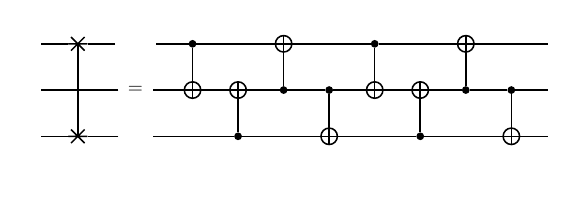
\begin{tikzpicture}
    \node[scale=0.7] {
    \begin{quantikz}
      \qw & \swap{2} & \qw \midstick[3,brackets=none]{=} & \ctrl{1} & \qw &\targ{}& \qw & \ctrl{1}& \qw &\targ & \qw & \qw & \qw \\
      \qw & \qw & \qw & \targ{} & \targ{} & \ctrl{-1} & \ctrl{1} & \targ{} & \targ{} & \ctrl{-1} & \ctrl{1} & \qw \\
      \qw & \swap{} & \qw & \qw & \ctrl{-1} & \qw &\targ{}& \qw & \ctrl{-1}& \qw &\targ & \qw & \qw \\
    \end{quantikz} };
  \end{tikzpicture}
  \caption{Simplifying three SWAP gates}
  \label{ex:swap-swap-decomposition}
\end{figure}

\begin{figure}[ht]
  \centering
  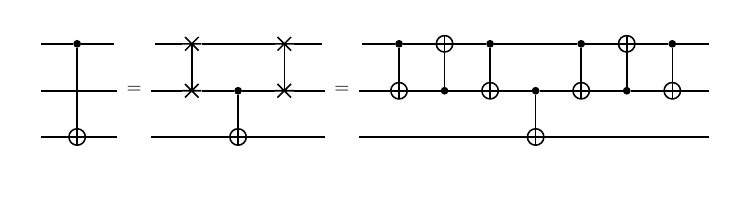
\begin{tikzpicture}
  \node[scale=0.7] {
  \begin{quantikz}
    \qw & \ctrl{2} & \qw \midstick[3,brackets=none]{=} & \swap{1} & \qw & \swap{1} & \qw \midstick[3,brackets=none]{=} & \ctrl{1} & \targ{} & \ctrl{1} & \qw &\ctrl{1} & \targ{} & \ctrl{1} & \qw \\
    \qw & \qw & \qw & \swap{} & \ctrl{1} & \swap{} & \qw & \targ{} & \ctrl{-1}& \targ{} & \ctrl{1} & \targ{} & \ctrl{-1}& \targ{} & \qw \\
    \qw & \targ{} & \qw  & \qw & \targ{} & \qw & \qw & \qw & \qw & \qw & \targ & \qw & \qw & \qw & \qw  & \qw \\
    \end{quantikz}
  };
  \end{tikzpicture} \\
  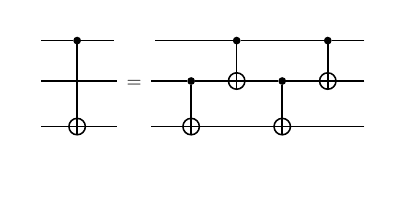
\begin{tikzpicture}
    \node[scale=0.7] {
    \begin{quantikz}
    \qw & \ctrl{2} & \qw \midstick[3,brackets=none]{=} & \qw & \ctrl{1} & \qw & \ctrl{1} & \qw \\
    \qw & \qw & \qw & \ctrl{1} & \targ{} & \ctrl{1}  & \targ{} & \qw \\
    \qw & \targ{} & \qw & \targ{} & \qw  & \targ & \qw  & \qw &  \qw \\
    \end{quantikz}
    };
  \end{tikzpicture}

  \caption{Simplifying a CNOT bridge}
  \label{ex:cnot-bridge-decomposition}
\end{figure}

In order to generalize this idea, we define the following problem

\begin{problem}[Bridging two-qubit gates]
  The solution to the problem of Bridging two-qubit gate $U$ over $n$ qubits is a circuit that can be applied on $n + 2$ qubits such that the $n$ qubits in the middle are not affected and the two qubits on the ends are mapped with respect to $U$. The circuit should normally obey a connectivity and a gate set constraints.
\end{problem}

Note that this definition is valid for classical case as well. In this case, the gate $U$ is a classical reversible gate applying on bits instead of qubits.

\section{Classical Bridging}\label{sec:classical_bridging}

Quantum logical circuits or classical reversible circuits are a class of circuits that are in common between classical and quantum computation. This class has been defined carefuly \cite{shende2006} and it has been proven that any classical reversible circuit can be synthesized using $X$ (classically known as NOT), CNOT and TOFFOLI gates.

Two-bit classical gates are limited to identity, CNOT (in both directions) and SWAP upto local isomorphism (NOT gates).

We will show that CNOT could be bridged over $n$ qubits using $4n + O(1)$ CNOTs within the depth of $2n + O(1)$. Then, we can prove that not only this is result is optimal, but also SWAP has an optimal bound $3n + O(1)$ CNOTs and $3n + O(1)$ depth that is already fulfilled by a simple decomposition.

\begin{theorem}
  Bridging CNOT($a$, $b$) over $n$ bits needs at least $4n$ CNOTs, where $n + 1$ must be the minimum distance between the two bits ($a$, $b$).
  \label{thm:bridging-cnot}
\end{theorem}
\begin{proof}
  We can layer the graph of bits in a way that the first layer is $a$, the last layer is $b$ and there are $n$ layers that we name any bit in layer $i$ as $c_i$. We also define right as the direction towards $b$ and left as th opposite direction.

  By considering a $\mathbb{F}_2$ vector space with hamming inner product $\langle \cdot, \cdot \rangle$ over the bits,  while each bit at each time has a unique vector, we can see that each CNOT as a linear operation adding a vector to another.

  If we name the set of every vector that is associated with a CNOT from layer $i$ to layer $i+1$ with $F_{i\rightarrow i+1}$ and simliarly $F_{i\leftarrow i+1}$, from the fact that the vector $a$ is going to be added to $b$ at the end, we know that the vector $a$ could be extracted from $F_{i\rightarrow i+1}$, which means that $a \in \mathrm{span}(F_{i\rightarrow i+1})$. On the other hand, in order to layer $i$ be unchanged after the process $\sum_{F_{i\leftarrow i+1}} f + \sum_{F_{i-1 \rightarrow i}} f = 0$.
  Mathematically, we can conclude from these two fact that one of these two cases hold for each layer $i$:

  Case 1 ($P(i)$): $F_{i\rightarrow i+1} = D \cup D'$ where $D \cap D' = \emptyset$ and $a \in \mathrm{span}(D)$ and $a \in \mathrm{span}(D')$.

  Case 2 ($Q(i)$): exists $f$ that $\langle f, a\rangle = 1$ and $f \in F_{i+1 \leftarrow i+2}$. 

  We separately prove that for the first case 
  \begin{equation}
    \abs{F_{i \rightarrow i+1}} + \abs{F_{i-1 \leftarrow i}} \geq 4
  \end{equation}
  and for the second case
  \begin{equation}
    \abs{F_{i+1 \rightarrow i+2}} + \abs{F_{i+1 \leftarrow i+2}} \geq 4
  \end{equation}

  Moreover we prove that $P(k+1)$ and $Q(k)$ cannot happen at the same time. This means that if $Q(k)$ holds, $Q(j)$ holds for all $j \geq k$.

  Then assuming $Q(k)$ and $P(k-1)$, by summing up the bounds

  \begin{equation}
    \sum_{i=0}^{k-1} \abs{F_{i \rightarrow i+1}} + \abs{F_{i-1 \leftarrow i}} + \sum_{i=k}^{n-2} \abs{F_{i+1 \rightarrow i+2}} + \abs{F_{i+1 \leftarrow i+2}} \geq 4n - O(1)
  \end{equation}

  This is due to the fact that these two summations has $O(1)$ terms in common. This means that the total number of CNOTs is at least $4n + O(1)$.
\end{proof}

\begin{lemma}[Bound for $P(i)$]
  For the first case used in the proof of Theorem~\ref{thm:bridging-cnot}, we have 
  \begin{equation}
    \abs{F_{i \rightarrow i+1}} + \abs{F_{i-1 \leftarrow i}} \geq 4
  \end{equation}
\end{lemma}
\begin{proof}
  If we call any arbitrary bit in $i$th layer by $c_i$, we know if $a \in F_{i \rightarrow i + 1}$,then it means that there was CNOTs, involving in removing $c_i$ from its site and returning it back. By a simple argument of capacity (in bits) the data could only be stored in the left-hand-side of $i$ meaning that vectors with $c_i$ element appeared in each of $F_{i-1 \leftarrow i}$ $F_{i-1 \rightarrow i}$ twice.

  Now, we already assumed that $a \in \mathrm{span}(D)$ and $a \in \mathrm{span}(D')$. 

  Case 1a: If $a \in D$ or $a \in D'$, then $a \in F_{i \rightarrow {i+1}}$. From the argument above we know that the vectors containing $c_i$ appear twice in $F_{i-1 \leftarrow i}$. One could easily conclude that $\abs{F_{i \rightarrow i+1}} + \abs{F_{i-1 \leftarrow i}} \geq 4$. 

  Case 1b: If $a \notin D$ and $a \notin D'$, then both $D$ and $D'$ need to have two vectors to have $a$ in their span, meaning $\abs{F_{i \rightarrow i+1}} \geq 4$.
\end{proof}

\begin{lemma}[Bound for $Q(i)$]
  For the second case used in the proof of Theorem~\ref{thm:bridging-cnot}, we have 
  \begin{equation}
    \abs{F_{i+1 \rightarrow i+2}} + \abs{F_{i+1 \leftarrow i+2}} \geq 4
  \end{equation}
\end{lemma}
\begin{proof}
  We know that $f \in F_{i+1 \rightarrow i+2}$ that $\langle f, a \rangle = 1$, in addition to that, $
  a \in \mathrm{span}(F_{i \rightarrow i+1})$ and independently $a \in \mathrm{span}(F_{i+1 \leftarrow i+2})$.

  If $\langle f, c_{i+2} \rangle = 0$ it means that $c_{i+2}$ must appear twice in each $F_{i+1 \rightarrow i+2}$ and $F_{i+1 \leftarrow i+2}$, so $F_{i+1 \rightarrow i+2} + F_{i+1 \leftarrow i+2} \geq 4$.

  Otherwise if $\langle f, c_{i+2} \rangle = 1$, then $c_{i+2}$ appears once in $F_{i+1 \leftarrow i+2}$. Noting the order of CNOTs, it must be before CNOTs associated with $a$, therefore all of the terms in $F_{i+1 \rightarrow i+2}$ with $a$ must have $c_{i+2}$ component as well. This makes impossible to $a \in F_{i+1 \rightarrow i+2}$. So $a \in \mathrm{span}(F_{i+1 \rightarrow i+2})$ results in $a$ appears twice, so $\abs{F_{i+1 \rightarrow i+2}} \geq 2$. Putting all together, $\abs{F_{i+1 \rightarrow i+2}} + \abs{F_{i+1 \leftarrow i+2}} \geq 4$.
\end{proof}

It could be easily shown that the circuit that is visualized in Figure \ref{fig:optimal-bridging-cnot} is an optimal solution for bridging CNOT.

\begin{figure}[ht]
  \centering
  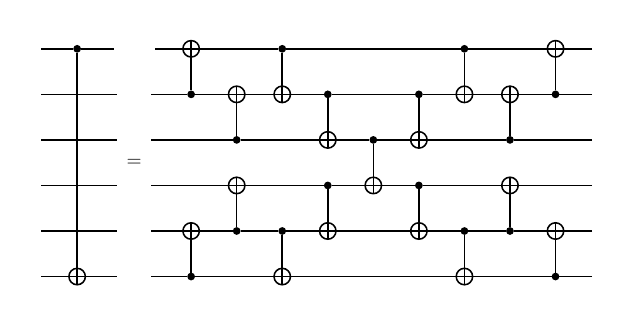
\begin{tikzpicture}
    \node[scale=0.7] {
      \begin{quantikz}
        \qw &\ctrl{5}&\qw \midstick[6,brackets=none]{=} &\targ{}  & \qw     &\ctrl{1}& \qw    & \qw    & \qw    &\ctrl{1}& \qw     &\targ{}&\qw\\
        \qw & \qw    & \qw    &\ctrl{-1}&\targ{}  & \targ{}&\ctrl{1}& \qw    &\ctrl{1}&\targ{} &\targ{}  &\ctrl{-1}&\qw\\
        \qw & \qw    & \qw    & \qw     &\ctrl{-1}& \qw    & \targ{}&\ctrl{1}&\targ{} & \qw    &\ctrl{-1}&\qw & \qw \\
        \qw & \qw    & \qw    & \qw     &\targ{}  & \qw    &\ctrl{1}& \targ{}&\ctrl{1}& \qw    &\targ{}  &\qw & \qw\\
        \qw & \qw    & \qw    &\targ{}  &\ctrl{-1}&\ctrl{1}& \targ{}& \qw    &\targ{} &\ctrl{1}&\ctrl{-1}&\targ{}&\qw \\
        \qw &\targ{} & \qw    &\ctrl{-1}& \qw     & \targ{}& \qw    & \qw    & \qw    &\targ{} & \qw     &\ctrl{-1}& \qw 
        \end{quantikz} };
  \end{tikzpicture}
  \caption{Optimal bridging CNOT}
  \label{fig:optimal-bridging-cnot}
\end{figure}

TODO: Show that two TOFFOLIs (with a NOT in between) are equal to a bridged CNOT over one bit.

TODO: Prove the optimality in presence of TOFFOLI in gate set.

\begin{theorem}
  Bridging SWAP($a$, $b$) over $n$ bits needs at least $6n$ CNOTs, where $n + 1$ must be the minimum distance between the two bits ($a$, $b$).
  \label{thm:bridging-swap}
\end{theorem}
\begin{proof}
  TODO
\end{proof}

\section{Quantum Bridging}

\begin{lemma}
  Any two-qubit gate with Schmidt number $2$ could be written as $L_1 \otimes L_2 CR_x(\theta) L_3 \otimes L_4$ where $L_i$ are local unitaries and $CR_x(\theta)$ is a controlled $R_x$ gate.
  \label{lem:decomposition-schmidt-2}
\end{lemma}
\begin{proof}
  Any two-qubit gate with Schmidt number $2$ could be written as $L_1 \otimes L_2 e^{i\alpha ZZ} L_3 \otimes L_4$. 
  Ignoring the local operations, by applying $R_z(-\theta)$ on the first and the second qubit, we will have 
  \begin{equation}
    R_z(-\theta) \otimes R_z(-\theta) e^{i\alpha ZZ} = CR_z(3\theta)
  \end{equation}
  
  that could be converted to $CR_x(\theta)$ by applying $H$ on the second qubit.
\end{proof}

\begin{theorem}[Optimal bridging For $CR_x$]
  Bridging $CR_x$ over $n$ qubits needs at least $4n$ CNOTs.
  \label{thm:bridging-crx}
\end{theorem}
\begin{proof}
  TODO
\end{proof}

\begin{theorem}[X-shaped bridge]
  

The circuit below, shows how to bridge any two-qubit gate with Schmidt number $2$ over $n$ qubits using $4n$ CNOTs and a $CR_x$.

\begin{figure}[ht]
  \centering
  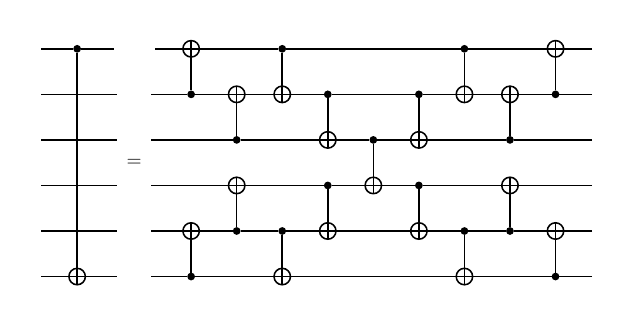
\begin{tikzpicture}
    \node[scale=0.7] {
      \begin{quantikz}
        \qw &\ctrl{5}&\qw \midstick[6,brackets=none]{=} &\targ{}  & \qw     &\ctrl{1}& \qw    & \qw    & \qw    &\ctrl{1}& \qw     &\targ{}&\qw\\
        \qw & \qw    & \qw    &\ctrl{-1}&\targ{}  & \targ{}&\ctrl{1}& \qw    &\ctrl{1}&\targ{} &\targ{}  &\ctrl{-1}&\qw\\
        \qw & \qw    & \qw    & \qw     &\ctrl{-1}& \qw    & \targ{}&\ctrl{1}&\targ{} & \qw    &\ctrl{-1}&\qw & \qw \\
        \qw & \qw    & \qw    & \qw     &\targ{}  & \qw    &\ctrl{1}& \targ{}&\ctrl{1}& \qw    &\targ{}  &\qw & \qw\\
        \qw & \qw    & \qw    &\targ{}  &\ctrl{-1}&\ctrl{1}& \targ{}& \qw    &\targ{} &\ctrl{1}&\ctrl{-1}&\targ{}&\qw \\
        \qw &\targ{} & \qw    &\ctrl{-1}& \qw     & \targ{}& \qw    & \qw    & \qw    &\targ{} & \qw     &\ctrl{-1}& \qw 
        \end{quantikz} };
  \end{tikzpicture}
  \caption{Optimal bridging CNOT}
  \label{fig:optimal-bridging-cnot}
\end{figure}

\chapter{Implementation}\label{chap:implementation}

TODO:
\begin{itemize}
  \item Qiskit: implementation in the routing stage \url{https://qiskit.org/documentation/apidoc/transpiler.html#routing-stage}
  \item tket: just test if it can do any of these simplifications
  \item PyZX (can do some of these simplifications)
\end{itemize}

\chapter{Conclusion}\label{chap:conclusion}

TODO

\printbibliography

\end{document}

